\documentclass[1p]{elsarticle_modified}
%\bibliographystyle{elsarticle-num}

%\usepackage[colorlinks]{hyperref}
%\usepackage{abbrmath_seonhwa} %\Abb, \Ascr, \Acal ,\Abf, \Afrak
\usepackage{amsfonts}
\usepackage{amssymb}
\usepackage{amsmath}
\usepackage{amsthm}
\usepackage{scalefnt}
\usepackage{amsbsy}
\usepackage{kotex}
\usepackage{caption}
\usepackage{subfig}
\usepackage{color}
\usepackage{graphicx}
\usepackage{xcolor} %% white, black, red, green, blue, cyan, magenta, yellow
\usepackage{float}
\usepackage{setspace}
\usepackage{hyperref}

\usepackage{tikz}
\usetikzlibrary{arrows}

\usepackage{multirow}
\usepackage{array} % fixed length table
\usepackage{hhline}

%%%%%%%%%%%%%%%%%%%%%
\makeatletter
\renewcommand*\env@matrix[1][\arraystretch]{%
	\edef\arraystretch{#1}%
	\hskip -\arraycolsep
	\let\@ifnextchar\new@ifnextchar
	\array{*\c@MaxMatrixCols c}}
\makeatother %https://tex.stackexchange.com/questions/14071/how-can-i-increase-the-line-spacing-in-a-matrix
%%%%%%%%%%%%%%%

\usepackage[normalem]{ulem}

\newcommand{\msout}[1]{\ifmmode\text{\sout{\ensuremath{#1}}}\else\sout{#1}\fi}
%SOURCE: \msout is \stkout macro in https://tex.stackexchange.com/questions/20609/strikeout-in-math-mode

\newcommand{\cancel}[1]{
	\ifmmode
	{\color{red}\msout{#1}}
	\else
	{\color{red}\sout{#1}}
	\fi
}

\newcommand{\add}[1]{
	{\color{blue}\uwave{#1}}
}

\newcommand{\replace}[2]{
	\ifmmode
	{\color{red}\msout{#1}}{\color{blue}\uwave{#2}}
	\else
	{\color{red}\sout{#1}}{\color{blue}\uwave{#2}}
	\fi
}

\newcommand{\Sol}{\mathcal{S}} %segment
\newcommand{\D}{D} %diagram
\newcommand{\A}{\mathcal{A}} %arc


%%%%%%%%%%%%%%%%%%%%%%%%%%%%%5 test

\def\sl{\operatorname{\textup{SL}}(2,\Cbb)}
\def\psl{\operatorname{\textup{PSL}}(2,\Cbb)}
\def\quan{\mkern 1mu \triangleright \mkern 1mu}

\theoremstyle{definition}
\newtheorem{thm}{Theorem}[section]
\newtheorem{prop}[thm]{Proposition}
\newtheorem{lem}[thm]{Lemma}
\newtheorem{ques}[thm]{Question}
\newtheorem{cor}[thm]{Corollary}
\newtheorem{defn}[thm]{Definition}
\newtheorem{exam}[thm]{Example}
\newtheorem{rmk}[thm]{Remark}
\newtheorem{alg}[thm]{Algorithm}

\newcommand{\I}{\sqrt{-1}}
\begin{document}

%\begin{frontmatter}
%
%\title{Boundary parabolic representations of knots up to 8 crossings}
%
%%% Group authors per affiliation:
%\author{Yunhi Cho} 
%\address{Department of Mathematics, University of Seoul, Seoul, Korea}
%\ead{yhcho@uos.ac.kr}
%
%
%\author{Seonhwa Kim} %\fnref{s_kim}}
%\address{Center for Geometry and Physics, Institute for Basic Science, Pohang, 37673, Korea}
%\ead{ryeona17@ibs.re.kr}
%
%\author{Hyuk Kim}
%\address{Department of Mathematical Sciences, Seoul National University, Seoul 08826, Korea}
%\ead{hyukkim@snu.ac.kr}
%
%\author{Seokbeom Yoon}
%\address{Department of Mathematical Sciences, Seoul National University, Seoul, 08826,  Korea}
%\ead{sbyoon15@snu.ac.kr}
%
%\begin{abstract}
%We find all boundary parabolic representation of knots up to 8 crossings.
%
%\end{abstract}
%\begin{keyword}
%    \MSC[2010] 57M25 
%\end{keyword}
%
%\end{frontmatter}

%\linenumbers
%\tableofcontents
%
\newcommand\colored[1]{\textcolor{white}{\rule[-0.35ex]{0.8em}{1.4ex}}\kern-0.8em\color{red} #1}%
%\newcommand\colored[1]{\textcolor{white}{ #1}\kern-2.17ex	\textcolor{white}{ #1}\kern-1.81ex	\textcolor{white}{ #1}\kern-2.15ex\color{red}#1	}

{\Large $\underline{12a_{0321}~(K12a_{0321})}$}

\setlength{\tabcolsep}{10pt}
\renewcommand{\arraystretch}{1.6}
\vspace{1cm}\begin{tabular}{m{100pt}>{\centering\arraybackslash}m{274pt}}
\multirow{5}{120pt}{
	\centering
	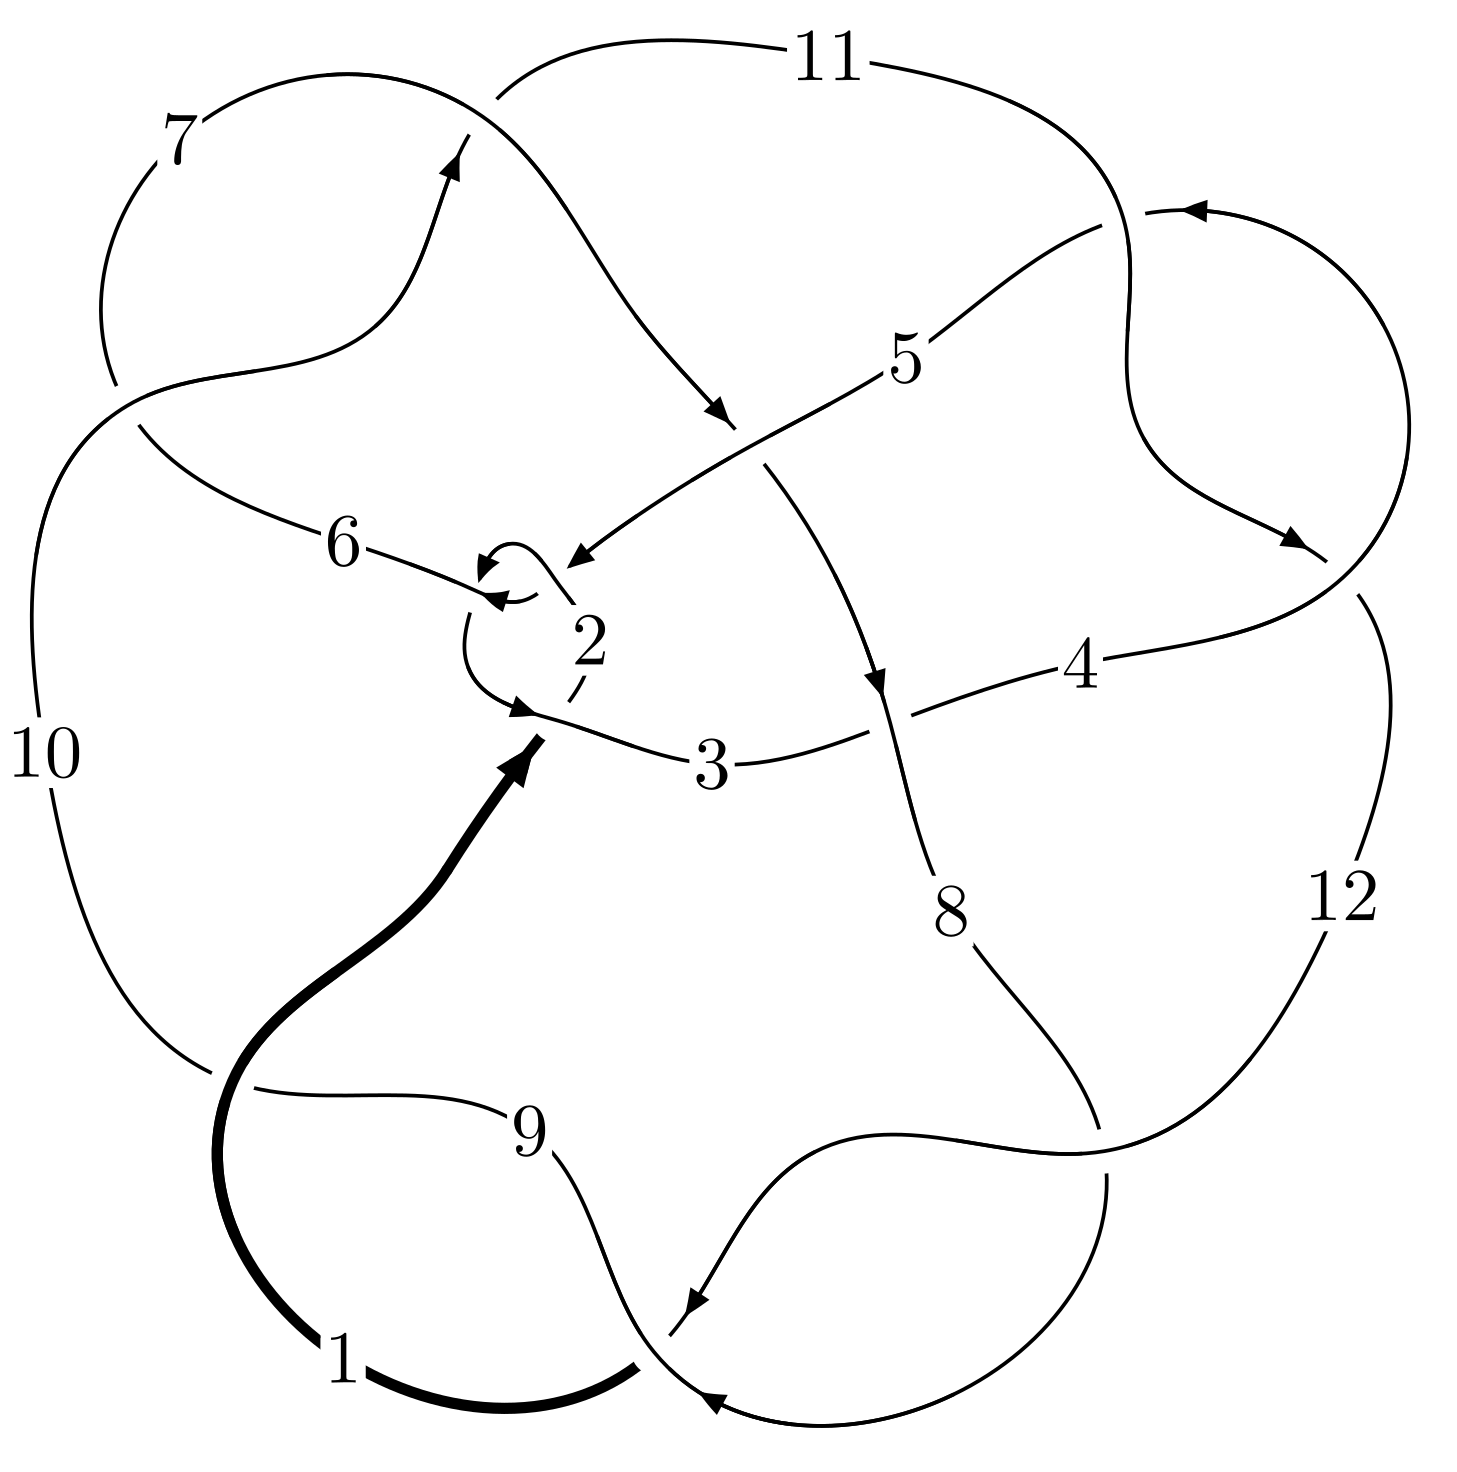
\includegraphics[width=112pt]{../../../GIT/diagram.site/Diagrams/png/1122_12a_0321.png}\\
\ \ \ A knot diagram\footnotemark}&
\allowdisplaybreaks
\textbf{Linearized knot diagam} \\
\cline{2-2}
 &
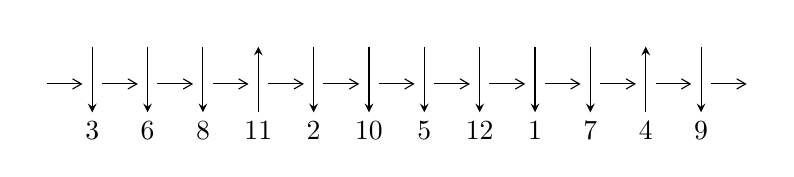
\begin{tikzpicture}[x=20pt, y=17pt]
	% nodes
	\node (C0) at (0, 0) {};
	\node (C1) at (1, 0) {};
	\node (C1U) at (1, +1) {};
	\node (C1D) at (1, -1) {3};

	\node (C2) at (2, 0) {};
	\node (C2U) at (2, +1) {};
	\node (C2D) at (2, -1) {6};

	\node (C3) at (3, 0) {};
	\node (C3U) at (3, +1) {};
	\node (C3D) at (3, -1) {8};

	\node (C4) at (4, 0) {};
	\node (C4U) at (4, +1) {};
	\node (C4D) at (4, -1) {11};

	\node (C5) at (5, 0) {};
	\node (C5U) at (5, +1) {};
	\node (C5D) at (5, -1) {2};

	\node (C6) at (6, 0) {};
	\node (C6U) at (6, +1) {};
	\node (C6D) at (6, -1) {10};

	\node (C7) at (7, 0) {};
	\node (C7U) at (7, +1) {};
	\node (C7D) at (7, -1) {5};

	\node (C8) at (8, 0) {};
	\node (C8U) at (8, +1) {};
	\node (C8D) at (8, -1) {12};

	\node (C9) at (9, 0) {};
	\node (C9U) at (9, +1) {};
	\node (C9D) at (9, -1) {1};

	\node (C10) at (10, 0) {};
	\node (C10U) at (10, +1) {};
	\node (C10D) at (10, -1) {7};

	\node (C11) at (11, 0) {};
	\node (C11U) at (11, +1) {};
	\node (C11D) at (11, -1) {4};

	\node (C12) at (12, 0) {};
	\node (C12U) at (12, +1) {};
	\node (C12D) at (12, -1) {9};
	\node (C13) at (13, 0) {};

	% arrows
	\draw[->,>={angle 60}]
	(C0) edge (C1) (C1) edge (C2) (C2) edge (C3) (C3) edge (C4) (C4) edge (C5) (C5) edge (C6) (C6) edge (C7) (C7) edge (C8) (C8) edge (C9) (C9) edge (C10) (C10) edge (C11) (C11) edge (C12) (C12) edge (C13) ;	\draw[->,>=stealth]
	(C1U) edge (C1D) (C2U) edge (C2D) (C3U) edge (C3D) (C4D) edge (C4U) (C5U) edge (C5D) (C6U) edge (C6D) (C7U) edge (C7D) (C8U) edge (C8D) (C9U) edge (C9D) (C10U) edge (C10D) (C11D) edge (C11U) (C12U) edge (C12D) ;
	\end{tikzpicture} \\
\hhline{~~} \\& 
\textbf{Solving Sequence} \\ \cline{2-2} 
 &
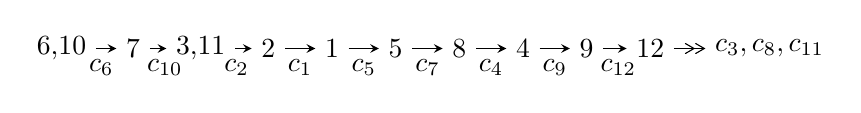
\begin{tikzpicture}[x=23pt, y=7pt]
	% node
	\node (A0) at (-1/8, 0) {6,10};
	\node (A1) at (1, 0) {7};
	\node (A2) at (33/16, 0) {3,11};
	\node (A3) at (25/8, 0) {2};
	\node (A4) at (33/8, 0) {1};
	\node (A5) at (41/8, 0) {5};
	\node (A6) at (49/8, 0) {8};
	\node (A7) at (57/8, 0) {4};
	\node (A8) at (65/8, 0) {9};
	\node (A9) at (73/8, 0) {12};
	\node (C1) at (1/2, -1) {$c_{6}$};
	\node (C2) at (3/2, -1) {$c_{10}$};
	\node (C3) at (21/8, -1) {$c_{2}$};
	\node (C4) at (29/8, -1) {$c_{1}$};
	\node (C5) at (37/8, -1) {$c_{5}$};
	\node (C6) at (45/8, -1) {$c_{7}$};
	\node (C7) at (53/8, -1) {$c_{4}$};
	\node (C8) at (61/8, -1) {$c_{9}$};
	\node (C9) at (69/8, -1) {$c_{12}$};
	\node (A10) at (11, 0) {$c_{3},c_{8},c_{11}$};

	% edge
	\draw[->,>=stealth]	
	(A0) edge (A1) (A1) edge (A2) (A2) edge (A3) (A3) edge (A4) (A4) edge (A5) (A5) edge (A6) (A6) edge (A7) (A7) edge (A8) (A8) edge (A9) ;
	\draw[->>,>={angle 60}]	
	(A9) edge (A10);
\end{tikzpicture} \\ 

\end{tabular} \\

\footnotetext{
The image of knot diagram is generated by the software ``\textbf{Draw programme}" developed by Andrew Bartholomew(\url{http://www.layer8.co.uk/maths/draw/index.htm\#Running-draw}), where we modified some parts for our purpose(\url{https://github.com/CATsTAILs/LinksPainter}).
}\phantom \\ \newline 
\centering \textbf{Ideals for irreducible components\footnotemark of $X_{\text{par}}$} 
 
\begin{align*}
I^u_{1}&=\langle 
-1.99007\times10^{472} u^{108}+6.02795\times10^{472} u^{107}+\cdots+7.29945\times10^{473} b+1.94243\times10^{476},\\
\phantom{I^u_{1}}&\phantom{= \langle  }1.10968\times10^{476} u^{108}-2.92557\times10^{476} u^{107}+\cdots+7.29288\times10^{477} a-1.87345\times10^{480},\\
\phantom{I^u_{1}}&\phantom{= \langle  }u^{109}-2 u^{108}+\cdots-109940 u-9991\rangle \\
I^u_{2}&=\langle 
-25716144203 u^{24}-112935246648 u^{23}+\cdots+50148875831 b+138327033199,\\
\phantom{I^u_{2}}&\phantom{= \langle  }80137258579 u^{24}+357502315466 u^{23}+\cdots+50148875831 a-608633590610,\\
\phantom{I^u_{2}}&\phantom{= \langle  }u^{25}+4 u^{24}+\cdots-8 u+1\rangle \\
I^u_{3}&=\langle 
b+1,\;a+2,\;u-1\rangle \\
\\
\end{align*}
\raggedright * 3 irreducible components of $\dim_{\mathbb{C}}=0$, with total 135 representations.\\
\footnotetext{All coefficients of polynomials are rational numbers. But the coefficients are sometimes approximated in decimal forms when there is not enough margin.}
\newpage
\renewcommand{\arraystretch}{1}
\centering \section*{I. $I^u_{1}= \langle -1.99\times10^{472} u^{108}+6.03\times10^{472} u^{107}+\cdots+7.30\times10^{473} b+1.94\times10^{476},\;1.11\times10^{476} u^{108}-2.93\times10^{476} u^{107}+\cdots+7.29\times10^{477} a-1.87\times10^{480},\;u^{109}-2 u^{108}+\cdots-109940 u-9991 \rangle$}
\flushleft \textbf{(i) Arc colorings}\\
\begin{tabular}{m{7pt} m{180pt} m{7pt} m{180pt} }
\flushright $a_{6}=$&$\begin{pmatrix}1\\0\end{pmatrix}$ \\
\flushright $a_{10}=$&$\begin{pmatrix}0\\u\end{pmatrix}$ \\
\flushright $a_{7}=$&$\begin{pmatrix}1\\u^2\end{pmatrix}$ \\
\flushright $a_{3}=$&$\begin{pmatrix}-0.0152159 u^{108}+0.0401154 u^{107}+\cdots+2397.87 u+256.887\\0.0272632 u^{108}-0.0825809 u^{107}+\cdots-2662.37 u-266.107\end{pmatrix}$ \\
\flushright $a_{11}=$&$\begin{pmatrix}- u\\- u^3+u\end{pmatrix}$ \\
\flushright $a_{2}=$&$\begin{pmatrix}0.0120473 u^{108}-0.0424655 u^{107}+\cdots-264.498 u-9.21983\\0.0272632 u^{108}-0.0825809 u^{107}+\cdots-2662.37 u-266.107\end{pmatrix}$ \\
\flushright $a_{1}=$&$\begin{pmatrix}-0.0309536 u^{108}+0.0971956 u^{107}+\cdots+2759.58 u+267.809\\0.0291866 u^{108}-0.0948676 u^{107}+\cdots-1781.19 u-152.041\end{pmatrix}$ \\
\flushright $a_{5}=$&$\begin{pmatrix}-0.0360067 u^{108}+0.116129 u^{107}+\cdots+2679.86 u+247.676\\-0.0501905 u^{108}+0.151970 u^{107}+\cdots+5267.74 u+535.227\end{pmatrix}$ \\
\flushright $a_{8}=$&$\begin{pmatrix}-0.0121877 u^{108}+0.0321171 u^{107}+\cdots+1791.13 u+187.009\\-0.0198379 u^{108}+0.0648994 u^{107}+\cdots+1260.31 u+108.071\end{pmatrix}$ \\
\flushright $a_{4}=$&$\begin{pmatrix}0.00315228 u^{108}-0.00784644 u^{107}+\cdots-853.506 u-104.441\\-0.0345567 u^{108}+0.100254 u^{107}+\cdots+4172.79 u+431.183\end{pmatrix}$ \\
\flushright $a_{9}=$&$\begin{pmatrix}0.0243292 u^{108}-0.0776944 u^{107}+\cdots-1908.35 u-190.269\\-0.0436852 u^{108}+0.132054 u^{107}+\cdots+4815.21 u+501.459\end{pmatrix}$ \\
\flushright $a_{12}=$&$\begin{pmatrix}-0.0202956 u^{108}+0.0688861 u^{107}+\cdots+1125.32 u+103.804\\-0.0285451 u^{108}+0.0917335 u^{107}+\cdots+2214.88 u+212.091\end{pmatrix}$\\&\end{tabular}
\flushleft \textbf{(ii) Obstruction class $= -1$}\\~\\
\flushleft \textbf{(iii) Cusp Shapes $= 0.0628061 u^{108}-0.159694 u^{107}+\cdots-11604.2 u-1313.19$}\\~\\
\newpage\renewcommand{\arraystretch}{1}
\flushleft \textbf{(iv) u-Polynomials at the component}\newline \\
\begin{tabular}{m{50pt}|m{274pt}}
Crossings & \hspace{64pt}u-Polynomials at each crossing \\
\hline $$\begin{aligned}c_{1}\end{aligned}$$&$\begin{aligned}
&u^{109}+53 u^{108}+\cdots+114 u+1
\end{aligned}$\\
\hline $$\begin{aligned}c_{2},c_{5}\end{aligned}$$&$\begin{aligned}
&u^{109}+5 u^{108}+\cdots+18 u+1
\end{aligned}$\\
\hline $$\begin{aligned}c_{3}\end{aligned}$$&$\begin{aligned}
&u^{109}+3 u^{108}+\cdots+9062344 u+742717
\end{aligned}$\\
\hline $$\begin{aligned}c_{4},c_{11}\end{aligned}$$&$\begin{aligned}
&u^{109}-4 u^{108}+\cdots+10 u-1
\end{aligned}$\\
\hline $$\begin{aligned}c_{6},c_{10}\end{aligned}$$&$\begin{aligned}
&u^{109}-2 u^{108}+\cdots-109940 u-9991
\end{aligned}$\\
\hline $$\begin{aligned}c_{7}\end{aligned}$$&$\begin{aligned}
&u^{109}-7 u^{108}+\cdots-1323756 u+105511
\end{aligned}$\\
\hline $$\begin{aligned}c_{8},c_{9},c_{12}\end{aligned}$$&$\begin{aligned}
&u^{109}+3 u^{108}+\cdots+95 u-7
\end{aligned}$\\
\hline
\end{tabular}\\~\\
\newpage\renewcommand{\arraystretch}{1}
\flushleft \textbf{(v) Riley Polynomials at the component}\newline \\
\begin{tabular}{m{50pt}|m{274pt}}
Crossings & \hspace{64pt}Riley Polynomials at each crossing \\
\hline $$\begin{aligned}c_{1}\end{aligned}$$&$\begin{aligned}
&y^{109}+19 y^{108}+\cdots+7262 y-1
\end{aligned}$\\
\hline $$\begin{aligned}c_{2},c_{5}\end{aligned}$$&$\begin{aligned}
&y^{109}-53 y^{108}+\cdots+114 y-1
\end{aligned}$\\
\hline $$\begin{aligned}c_{3}\end{aligned}$$&$\begin{aligned}
&y^{109}-47 y^{108}+\cdots+31084038325668 y-551628542089
\end{aligned}$\\
\hline $$\begin{aligned}c_{4},c_{11}\end{aligned}$$&$\begin{aligned}
&y^{109}+100 y^{108}+\cdots+112 y-1
\end{aligned}$\\
\hline $$\begin{aligned}c_{6},c_{10}\end{aligned}$$&$\begin{aligned}
&y^{109}-92 y^{108}+\cdots+1884094310 y-99820081
\end{aligned}$\\
\hline $$\begin{aligned}c_{7}\end{aligned}$$&$\begin{aligned}
&y^{109}-35 y^{108}+\cdots+312381658400 y-11132571121
\end{aligned}$\\
\hline $$\begin{aligned}c_{8},c_{9},c_{12}\end{aligned}$$&$\begin{aligned}
&y^{109}-117 y^{108}+\cdots-537 y-49
\end{aligned}$\\
\hline
\end{tabular}\\~\\
\newpage\flushleft \textbf{(vi) Complex Volumes and Cusp Shapes}
$$\begin{array}{c|c|c}  
\text{Solutions to }I^u_{1}& \I (\text{vol} + \sqrt{-1}CS) & \text{Cusp shape}\\
 \hline 
\begin{aligned}
u &= -0.927360 + 0.368807 I \\
a &= -0.004486 + 0.281853 I \\
b &= \phantom{-}0.541893 + 0.407683 I\end{aligned}
 & -0.881908 - 0.499794 I & \phantom{-0.000000 } 0 \\ \hline\begin{aligned}
u &= -0.927360 - 0.368807 I \\
a &= -0.004486 - 0.281853 I \\
b &= \phantom{-}0.541893 - 0.407683 I\end{aligned}
 & -0.881908 + 0.499794 I & \phantom{-0.000000 } 0 \\ \hline\begin{aligned}
u &= -0.001942 + 0.975609 I \\
a &= \phantom{-}0.359346 + 1.195970 I \\
b &= -0.532276 - 0.624869 I\end{aligned}
 & -0.33225 + 2.57093 I & \phantom{-0.000000 } 0 \\ \hline\begin{aligned}
u &= -0.001942 - 0.975609 I \\
a &= \phantom{-}0.359346 - 1.195970 I \\
b &= -0.532276 + 0.624869 I\end{aligned}
 & -0.33225 - 2.57093 I & \phantom{-0.000000 } 0 \\ \hline\begin{aligned}
u &= \phantom{-}1.057370 + 0.207259 I \\
a &= \phantom{-}0.024452 + 0.732775 I \\
b &= -0.631857 - 0.932609 I\end{aligned}
 & -3.02837 - 3.95297 I & \phantom{-0.000000 } 0 \\ \hline\begin{aligned}
u &= \phantom{-}1.057370 - 0.207259 I \\
a &= \phantom{-}0.024452 - 0.732775 I \\
b &= -0.631857 + 0.932609 I\end{aligned}
 & -3.02837 + 3.95297 I & \phantom{-0.000000 } 0 \\ \hline\begin{aligned}
u &= -0.892897 + 0.611548 I \\
a &= -0.498464 - 0.905635 I \\
b &= \phantom{-}0.661982 + 0.108547 I\end{aligned}
 & -4.68433 + 2.02276 I & \phantom{-0.000000 } 0 \\ \hline\begin{aligned}
u &= -0.892897 - 0.611548 I \\
a &= -0.498464 + 0.905635 I \\
b &= \phantom{-}0.661982 - 0.108547 I\end{aligned}
 & -4.68433 - 2.02276 I & \phantom{-0.000000 } 0 \\ \hline\begin{aligned}
u &= \phantom{-}1.08678\phantom{ +0.000000I} \\
a &= -1.37532\phantom{ +0.000000I} \\
b &= -1.15010\phantom{ +0.000000I}\end{aligned}
 & -4.90949\phantom{ +0.000000I} & \phantom{-0.000000 } 0 \\ \hline\begin{aligned}
u &= -0.141033 + 1.081570 I \\
a &= -0.735304 - 0.856968 I \\
b &= \phantom{-}1.115130 + 0.539463 I\end{aligned}
 & -4.62116 - 6.15750 I & \phantom{-0.000000 } 0\\
 \hline 
 \end{array}$$\newpage$$\begin{array}{c|c|c}  
\text{Solutions to }I^u_{1}& \I (\text{vol} + \sqrt{-1}CS) & \text{Cusp shape}\\
 \hline 
\begin{aligned}
u &= -0.141033 - 1.081570 I \\
a &= -0.735304 + 0.856968 I \\
b &= \phantom{-}1.115130 - 0.539463 I\end{aligned}
 & -4.62116 + 6.15750 I & \phantom{-0.000000 } 0 \\ \hline\begin{aligned}
u &= \phantom{-}1.042030 + 0.340775 I \\
a &= -0.342757 + 0.367631 I \\
b &= \phantom{-}0.307587 - 0.839493 I\end{aligned}
 & \phantom{-}0.59322 - 2.98567 I & \phantom{-0.000000 } 0 \\ \hline\begin{aligned}
u &= \phantom{-}1.042030 - 0.340775 I \\
a &= -0.342757 - 0.367631 I \\
b &= \phantom{-}0.307587 + 0.839493 I\end{aligned}
 & \phantom{-}0.59322 + 2.98567 I & \phantom{-0.000000 } 0 \\ \hline\begin{aligned}
u &= \phantom{-}0.481404 + 0.728442 I \\
a &= \phantom{-}1.58446 - 0.53180 I \\
b &= -1.077880 + 0.314975 I\end{aligned}
 & -6.22931 + 1.23975 I & \phantom{-0.000000 } 0 \\ \hline\begin{aligned}
u &= \phantom{-}0.481404 - 0.728442 I \\
a &= \phantom{-}1.58446 + 0.53180 I \\
b &= -1.077880 - 0.314975 I\end{aligned}
 & -6.22931 - 1.23975 I & \phantom{-0.000000 } 0 \\ \hline\begin{aligned}
u &= -0.164225 + 1.134570 I \\
a &= \phantom{-}0.234584 - 1.329010 I \\
b &= -1.001660 + 0.578622 I\end{aligned}
 & -1.68142 + 7.31001 I & \phantom{-0.000000 } 0 \\ \hline\begin{aligned}
u &= -0.164225 - 1.134570 I \\
a &= \phantom{-}0.234584 + 1.329010 I \\
b &= -1.001660 - 0.578622 I\end{aligned}
 & -1.68142 - 7.31001 I & \phantom{-0.000000 } 0 \\ \hline\begin{aligned}
u &= -1.146230 + 0.151412 I \\
a &= -0.421695 - 1.097710 I \\
b &= -1.39389 + 0.83781 I\end{aligned}
 & -10.94360 + 3.34958 I & \phantom{-0.000000 } 0 \\ \hline\begin{aligned}
u &= -1.146230 - 0.151412 I \\
a &= -0.421695 + 1.097710 I \\
b &= -1.39389 - 0.83781 I\end{aligned}
 & -10.94360 - 3.34958 I & \phantom{-0.000000 } 0 \\ \hline\begin{aligned}
u &= -1.117690 + 0.324951 I \\
a &= -0.82076 - 1.63481 I \\
b &= -1.040340 + 0.440134 I\end{aligned}
 & -2.81887 + 3.16219 I & \phantom{-0.000000 } 0\\
 \hline 
 \end{array}$$\newpage$$\begin{array}{c|c|c}  
\text{Solutions to }I^u_{1}& \I (\text{vol} + \sqrt{-1}CS) & \text{Cusp shape}\\
 \hline 
\begin{aligned}
u &= -1.117690 - 0.324951 I \\
a &= -0.82076 + 1.63481 I \\
b &= -1.040340 - 0.440134 I\end{aligned}
 & -2.81887 - 3.16219 I & \phantom{-0.000000 } 0 \\ \hline\begin{aligned}
u &= -1.171050 + 0.062575 I \\
a &= \phantom{-}0.243573 - 0.861666 I \\
b &= -0.75611 + 1.19829 I\end{aligned}
 & -8.95265 + 4.63111 I & \phantom{-0.000000 } 0 \\ \hline\begin{aligned}
u &= -1.171050 - 0.062575 I \\
a &= \phantom{-}0.243573 + 0.861666 I \\
b &= -0.75611 - 1.19829 I\end{aligned}
 & -8.95265 - 4.63111 I & \phantom{-0.000000 } 0 \\ \hline\begin{aligned}
u &= \phantom{-}1.173030 + 0.041004 I \\
a &= -0.540423 + 0.900178 I \\
b &= -1.212730 - 0.663125 I\end{aligned}
 & -4.98444 - 2.41357 I & \phantom{-0.000000 } 0 \\ \hline\begin{aligned}
u &= \phantom{-}1.173030 - 0.041004 I \\
a &= -0.540423 - 0.900178 I \\
b &= -1.212730 + 0.663125 I\end{aligned}
 & -4.98444 + 2.41357 I & \phantom{-0.000000 } 0 \\ \hline\begin{aligned}
u &= -1.176150 + 0.036021 I \\
a &= \phantom{-}1.51938 - 1.46237 I \\
b &= \phantom{-}1.066390 + 0.426048 I\end{aligned}
 & -6.86041 - 0.88784 I & \phantom{-0.000000 } 0 \\ \hline\begin{aligned}
u &= -1.176150 - 0.036021 I \\
a &= \phantom{-}1.51938 + 1.46237 I \\
b &= \phantom{-}1.066390 - 0.426048 I\end{aligned}
 & -6.86041 + 0.88784 I & \phantom{-0.000000 } 0 \\ \hline\begin{aligned}
u &= \phantom{-}0.108220 + 1.194260 I \\
a &= -0.04457 - 1.44047 I \\
b &= -0.381359 + 0.662655 I\end{aligned}
 & -6.68074 - 5.67638 I & \phantom{-0.000000 } 0 \\ \hline\begin{aligned}
u &= \phantom{-}0.108220 - 1.194260 I \\
a &= -0.04457 + 1.44047 I \\
b &= -0.381359 - 0.662655 I\end{aligned}
 & -6.68074 + 5.67638 I & \phantom{-0.000000 } 0 \\ \hline\begin{aligned}
u &= -1.136990 + 0.387269 I \\
a &= -0.468289 - 0.722813 I \\
b &= \phantom{-}0.211741 + 1.127560 I\end{aligned}
 & -5.03193 + 5.61101 I & \phantom{-0.000000 } 0\\
 \hline 
 \end{array}$$\newpage$$\begin{array}{c|c|c}  
\text{Solutions to }I^u_{1}& \I (\text{vol} + \sqrt{-1}CS) & \text{Cusp shape}\\
 \hline 
\begin{aligned}
u &= -1.136990 - 0.387269 I \\
a &= -0.468289 + 0.722813 I \\
b &= \phantom{-}0.211741 - 1.127560 I\end{aligned}
 & -5.03193 - 5.61101 I & \phantom{-0.000000 } 0 \\ \hline\begin{aligned}
u &= \phantom{-}1.198400 + 0.113222 I \\
a &= \phantom{-}0.51876 - 1.94605 I \\
b &= \phantom{-}1.122610 + 0.582933 I\end{aligned}
 & -13.0830 - 7.0865 I & \phantom{-0.000000 } 0 \\ \hline\begin{aligned}
u &= \phantom{-}1.198400 - 0.113222 I \\
a &= \phantom{-}0.51876 + 1.94605 I \\
b &= \phantom{-}1.122610 - 0.582933 I\end{aligned}
 & -13.0830 + 7.0865 I & \phantom{-0.000000 } 0 \\ \hline\begin{aligned}
u &= \phantom{-}1.181720 + 0.307746 I \\
a &= \phantom{-}0.678893 - 0.995764 I \\
b &= -0.423479 + 0.760999 I\end{aligned}
 & -6.45027 - 1.36251 I & \phantom{-0.000000 } 0 \\ \hline\begin{aligned}
u &= \phantom{-}1.181720 - 0.307746 I \\
a &= \phantom{-}0.678893 + 0.995764 I \\
b &= -0.423479 - 0.760999 I\end{aligned}
 & -6.45027 + 1.36251 I & \phantom{-0.000000 } 0 \\ \hline\begin{aligned}
u &= -0.247531 + 0.733819 I \\
a &= \phantom{-}0.56761 + 1.55074 I \\
b &= \phantom{-}0.310446 - 0.709793 I\end{aligned}
 & -2.28524 - 1.40023 I & \phantom{-0.000000 } 0 \\ \hline\begin{aligned}
u &= -0.247531 - 0.733819 I \\
a &= \phantom{-}0.56761 - 1.55074 I \\
b &= \phantom{-}0.310446 + 0.709793 I\end{aligned}
 & -2.28524 + 1.40023 I & \phantom{-0.000000 } 0 \\ \hline\begin{aligned}
u &= \phantom{-}1.226970 + 0.097481 I \\
a &= -0.862780 - 0.648315 I \\
b &= \phantom{-}0.394183 + 0.774439 I\end{aligned}
 & -10.89780 + 1.94807 I & \phantom{-0.000000 } 0 \\ \hline\begin{aligned}
u &= \phantom{-}1.226970 - 0.097481 I \\
a &= -0.862780 + 0.648315 I \\
b &= \phantom{-}0.394183 - 0.774439 I\end{aligned}
 & -10.89780 - 1.94807 I & \phantom{-0.000000 } 0 \\ \hline\begin{aligned}
u &= \phantom{-}0.032475 + 0.748168 I \\
a &= -0.528278 + 1.089850 I \\
b &= \phantom{-}0.936740 - 0.608484 I\end{aligned}
 & \phantom{-}1.92695 + 3.99796 I & -3.21801 - 6.20905 I\\
 \hline 
 \end{array}$$\newpage$$\begin{array}{c|c|c}  
\text{Solutions to }I^u_{1}& \I (\text{vol} + \sqrt{-1}CS) & \text{Cusp shape}\\
 \hline 
\begin{aligned}
u &= \phantom{-}0.032475 - 0.748168 I \\
a &= -0.528278 - 1.089850 I \\
b &= \phantom{-}0.936740 + 0.608484 I\end{aligned}
 & \phantom{-}1.92695 - 3.99796 I & -3.21801 + 6.20905 I \\ \hline\begin{aligned}
u &= \phantom{-}0.316631 + 0.673261 I \\
a &= -0.040172 - 1.317730 I \\
b &= \phantom{-}0.661258 + 0.648032 I\end{aligned}
 & \phantom{-}2.74013 - 0.88698 I & \phantom{-0.000000 } 0 \\ \hline\begin{aligned}
u &= \phantom{-}0.316631 - 0.673261 I \\
a &= -0.040172 + 1.317730 I \\
b &= \phantom{-}0.661258 - 0.648032 I\end{aligned}
 & \phantom{-}2.74013 + 0.88698 I & \phantom{-0.000000 } 0 \\ \hline\begin{aligned}
u &= -1.25835\phantom{ +0.000000I} \\
a &= -0.260141\phantom{ +0.000000I} \\
b &= -1.65764\phantom{ +0.000000I}\end{aligned}
 & -11.9769\phantom{ +0.000000I} & \phantom{-0.000000 } 0 \\ \hline\begin{aligned}
u &= -0.733035\phantom{ +0.000000I} \\
a &= \phantom{-}0.648851\phantom{ +0.000000I} \\
b &= -0.107199\phantom{ +0.000000I}\end{aligned}
 & -0.968982\phantom{ +0.000000I} & -9.84640\phantom{ +0.000000I} \\ \hline\begin{aligned}
u &= \phantom{-}1.248920 + 0.255227 I \\
a &= \phantom{-}1.253130 + 0.044705 I \\
b &= \phantom{-}1.106620 - 0.157497 I\end{aligned}
 & -9.54974 - 5.10430 I & \phantom{-0.000000 } 0 \\ \hline\begin{aligned}
u &= \phantom{-}1.248920 - 0.255227 I \\
a &= \phantom{-}1.253130 - 0.044705 I \\
b &= \phantom{-}1.106620 + 0.157497 I\end{aligned}
 & -9.54974 + 5.10430 I & \phantom{-0.000000 } 0 \\ \hline\begin{aligned}
u &= -1.201150 + 0.436460 I \\
a &= -0.171617 - 0.684167 I \\
b &= -0.220383 + 0.206899 I\end{aligned}
 & -4.39780 + 2.11444 I & \phantom{-0.000000 } 0 \\ \hline\begin{aligned}
u &= -1.201150 - 0.436460 I \\
a &= -0.171617 + 0.684167 I \\
b &= -0.220383 - 0.206899 I\end{aligned}
 & -4.39780 - 2.11444 I & \phantom{-0.000000 } 0 \\ \hline\begin{aligned}
u &= -1.224520 + 0.378182 I \\
a &= \phantom{-}0.077221 - 0.365173 I \\
b &= -0.298317 - 0.328543 I\end{aligned}
 & -4.36955 + 2.20355 I & \phantom{-0.000000 } 0\\
 \hline 
 \end{array}$$\newpage$$\begin{array}{c|c|c}  
\text{Solutions to }I^u_{1}& \I (\text{vol} + \sqrt{-1}CS) & \text{Cusp shape}\\
 \hline 
\begin{aligned}
u &= -1.224520 - 0.378182 I \\
a &= \phantom{-}0.077221 + 0.365173 I \\
b &= -0.298317 + 0.328543 I\end{aligned}
 & -4.36955 - 2.20355 I & \phantom{-0.000000 } 0 \\ \hline\begin{aligned}
u &= \phantom{-}1.186760 + 0.526901 I \\
a &= \phantom{-}1.16922 - 1.11264 I \\
b &= \phantom{-}0.943150 + 0.121171 I\end{aligned}
 & -9.22014 - 5.07106 I & \phantom{-0.000000 } 0 \\ \hline\begin{aligned}
u &= \phantom{-}1.186760 - 0.526901 I \\
a &= \phantom{-}1.16922 + 1.11264 I \\
b &= \phantom{-}0.943150 - 0.121171 I\end{aligned}
 & -9.22014 + 5.07106 I & \phantom{-0.000000 } 0 \\ \hline\begin{aligned}
u &= -0.463740 + 0.510377 I \\
a &= \phantom{-}0.067072 - 1.240980 I \\
b &= \phantom{-}0.893561 - 0.026652 I\end{aligned}
 & -4.67096 + 1.93516 I & -15.9176 - 3.5896 I \\ \hline\begin{aligned}
u &= -0.463740 - 0.510377 I \\
a &= \phantom{-}0.067072 + 1.240980 I \\
b &= \phantom{-}0.893561 + 0.026652 I\end{aligned}
 & -4.67096 - 1.93516 I & -15.9176 + 3.5896 I \\ \hline\begin{aligned}
u &= -1.299780 + 0.179706 I \\
a &= \phantom{-}0.972081 + 0.717778 I \\
b &= \phantom{-}1.046880 - 0.479841 I\end{aligned}
 & -2.54445 + 3.37243 I & \phantom{-0.000000 } 0 \\ \hline\begin{aligned}
u &= -1.299780 - 0.179706 I \\
a &= \phantom{-}0.972081 - 0.717778 I \\
b &= \phantom{-}1.046880 + 0.479841 I\end{aligned}
 & -2.54445 - 3.37243 I & \phantom{-0.000000 } 0 \\ \hline\begin{aligned}
u &= \phantom{-}1.264240 + 0.390206 I \\
a &= \phantom{-}0.73496 - 1.23757 I \\
b &= \phantom{-}1.147500 + 0.584416 I\end{aligned}
 & -1.89007 - 8.23554 I & \phantom{-0.000000 } 0 \\ \hline\begin{aligned}
u &= \phantom{-}1.264240 - 0.390206 I \\
a &= \phantom{-}0.73496 + 1.23757 I \\
b &= \phantom{-}1.147500 - 0.584416 I\end{aligned}
 & -1.89007 + 8.23554 I & \phantom{-0.000000 } 0 \\ \hline\begin{aligned}
u &= \phantom{-}1.252170 + 0.558161 I \\
a &= -0.08507 + 1.67329 I \\
b &= -1.108000 - 0.585173 I\end{aligned}
 & -8.50772 - 6.47710 I & \phantom{-0.000000 } 0\\
 \hline 
 \end{array}$$\newpage$$\begin{array}{c|c|c}  
\text{Solutions to }I^u_{1}& \I (\text{vol} + \sqrt{-1}CS) & \text{Cusp shape}\\
 \hline 
\begin{aligned}
u &= \phantom{-}1.252170 - 0.558161 I \\
a &= -0.08507 - 1.67329 I \\
b &= -1.108000 + 0.585173 I\end{aligned}
 & -8.50772 + 6.47710 I & \phantom{-0.000000 } 0 \\ \hline\begin{aligned}
u &= -1.288050 + 0.518655 I \\
a &= \phantom{-}0.41587 + 1.40242 I \\
b &= \phantom{-}1.26484 - 0.63490 I\end{aligned}
 & -8.2774 + 11.7660 I & \phantom{-0.000000 } 0 \\ \hline\begin{aligned}
u &= -1.288050 - 0.518655 I \\
a &= \phantom{-}0.41587 - 1.40242 I \\
b &= \phantom{-}1.26484 + 0.63490 I\end{aligned}
 & -8.2774 - 11.7660 I & \phantom{-0.000000 } 0 \\ \hline\begin{aligned}
u &= \phantom{-}1.313920 + 0.456848 I \\
a &= \phantom{-}0.448450 - 0.453491 I \\
b &= -0.368355 + 0.821745 I\end{aligned}
 & -4.47485 - 7.63949 I & \phantom{-0.000000 } 0 \\ \hline\begin{aligned}
u &= \phantom{-}1.313920 - 0.456848 I \\
a &= \phantom{-}0.448450 + 0.453491 I \\
b &= -0.368355 - 0.821745 I\end{aligned}
 & -4.47485 + 7.63949 I & \phantom{-0.000000 } 0 \\ \hline\begin{aligned}
u &= -1.40284 + 0.26612 I \\
a &= -1.27343 - 0.81645 I \\
b &= -1.075530 + 0.475402 I\end{aligned}
 & -6.50588 + 6.06163 I & \phantom{-0.000000 } 0 \\ \hline\begin{aligned}
u &= -1.40284 - 0.26612 I \\
a &= -1.27343 + 0.81645 I \\
b &= -1.075530 - 0.475402 I\end{aligned}
 & -6.50588 - 6.06163 I & \phantom{-0.000000 } 0 \\ \hline\begin{aligned}
u &= -0.514954 + 0.241943 I \\
a &= \phantom{-}1.287940 + 0.250825 I \\
b &= -0.694966 - 0.159105 I\end{aligned}
 & -1.130220 - 0.058098 I & -6.31168 - 0.93824 I \\ \hline\begin{aligned}
u &= -0.514954 - 0.241943 I \\
a &= \phantom{-}1.287940 - 0.250825 I \\
b &= -0.694966 + 0.159105 I\end{aligned}
 & -1.130220 + 0.058098 I & -6.31168 + 0.93824 I \\ \hline\begin{aligned}
u &= -0.539163 + 0.088043 I \\
a &= -0.63521 + 1.61057 I \\
b &= \phantom{-}0.871250 - 0.779499 I\end{aligned}
 & \phantom{-}1.25521 + 2.92708 I & -20.6191 - 7.0979 I\\
 \hline 
 \end{array}$$\newpage$$\begin{array}{c|c|c}  
\text{Solutions to }I^u_{1}& \I (\text{vol} + \sqrt{-1}CS) & \text{Cusp shape}\\
 \hline 
\begin{aligned}
u &= -0.539163 - 0.088043 I \\
a &= -0.63521 - 1.61057 I \\
b &= \phantom{-}0.871250 + 0.779499 I\end{aligned}
 & \phantom{-}1.25521 - 2.92708 I & -20.6191 + 7.0979 I \\ \hline\begin{aligned}
u &= -0.136443 + 0.527344 I \\
a &= \phantom{-}1.68053 - 0.92025 I \\
b &= -0.723335 + 0.458886 I\end{aligned}
 & -0.79469 + 1.36894 I & -9.17150 - 4.18616 I \\ \hline\begin{aligned}
u &= -0.136443 - 0.527344 I \\
a &= \phantom{-}1.68053 + 0.92025 I \\
b &= -0.723335 - 0.458886 I\end{aligned}
 & -0.79469 - 1.36894 I & -9.17150 + 4.18616 I \\ \hline\begin{aligned}
u &= \phantom{-}0.85209 + 1.22980 I \\
a &= -0.664286 + 0.651414 I \\
b &= \phantom{-}1.051060 - 0.329189 I\end{aligned}
 & -10.33410 - 3.36596 I & \phantom{-0.000000 } 0 \\ \hline\begin{aligned}
u &= \phantom{-}0.85209 - 1.22980 I \\
a &= -0.664286 - 0.651414 I \\
b &= \phantom{-}1.051060 + 0.329189 I\end{aligned}
 & -10.33410 + 3.36596 I & \phantom{-0.000000 } 0 \\ \hline\begin{aligned}
u &= -0.374092 + 0.331035 I \\
a &= \phantom{-}1.032560 - 0.927902 I \\
b &= -1.142870 - 0.573781 I\end{aligned}
 & -8.60926 - 1.47993 I & -14.4229 + 2.1286 I \\ \hline\begin{aligned}
u &= -0.374092 - 0.331035 I \\
a &= \phantom{-}1.032560 + 0.927902 I \\
b &= -1.142870 + 0.573781 I\end{aligned}
 & -8.60926 + 1.47993 I & -14.4229 - 2.1286 I \\ \hline\begin{aligned}
u &= -1.48071 + 0.25387 I \\
a &= \phantom{-}0.319112 - 0.074073 I \\
b &= \phantom{-}1.404500 + 0.116946 I\end{aligned}
 & -18.0245 + 7.5939 I & \phantom{-0.000000 } 0 \\ \hline\begin{aligned}
u &= -1.48071 - 0.25387 I \\
a &= \phantom{-}0.319112 + 0.074073 I \\
b &= \phantom{-}1.404500 - 0.116946 I\end{aligned}
 & -18.0245 - 7.5939 I & \phantom{-0.000000 } 0 \\ \hline\begin{aligned}
u &= \phantom{-}0.480994 + 0.126570 I \\
a &= -1.96808 - 2.47848 I \\
b &= \phantom{-}1.076970 - 0.299233 I\end{aligned}
 & -10.61350 + 5.99402 I & -18.1018 - 3.7342 I\\
 \hline 
 \end{array}$$\newpage$$\begin{array}{c|c|c}  
\text{Solutions to }I^u_{1}& \I (\text{vol} + \sqrt{-1}CS) & \text{Cusp shape}\\
 \hline 
\begin{aligned}
u &= \phantom{-}0.480994 - 0.126570 I \\
a &= -1.96808 + 2.47848 I \\
b &= \phantom{-}1.076970 + 0.299233 I\end{aligned}
 & -10.61350 - 5.99402 I & -18.1018 + 3.7342 I \\ \hline\begin{aligned}
u &= \phantom{-}0.098496 + 0.483051 I \\
a &= \phantom{-}1.228410 + 0.028238 I \\
b &= -0.443278 + 0.446712 I\end{aligned}
 & -0.67889 + 1.28300 I & -6.58010 - 4.63125 I \\ \hline\begin{aligned}
u &= \phantom{-}0.098496 - 0.483051 I \\
a &= \phantom{-}1.228410 - 0.028238 I \\
b &= -0.443278 - 0.446712 I\end{aligned}
 & -0.67889 - 1.28300 I & -6.58010 + 4.63125 I \\ \hline\begin{aligned}
u &= \phantom{-}0.109455 + 0.479164 I \\
a &= -0.82993 + 1.99601 I \\
b &= -0.929731 - 0.602032 I\end{aligned}
 & -1.52384 - 3.08285 I & -9.69293 + 2.06484 I \\ \hline\begin{aligned}
u &= \phantom{-}0.109455 - 0.479164 I \\
a &= -0.82993 - 1.99601 I \\
b &= -0.929731 + 0.602032 I\end{aligned}
 & -1.52384 + 3.08285 I & -9.69293 - 2.06484 I \\ \hline\begin{aligned}
u &= -1.42468 + 0.49590 I \\
a &= \phantom{-}0.427632 + 0.788644 I \\
b &= -0.357295 - 1.022260 I\end{aligned}
 & -11.6087 + 11.5120 I & \phantom{-0.000000 } 0 \\ \hline\begin{aligned}
u &= -1.42468 - 0.49590 I \\
a &= \phantom{-}0.427632 - 0.788644 I \\
b &= -0.357295 + 1.022260 I\end{aligned}
 & -11.6087 - 11.5120 I & \phantom{-0.000000 } 0 \\ \hline\begin{aligned}
u &= -1.49024 + 0.24040 I \\
a &= -0.370784 + 0.651679 I \\
b &= -1.026120 - 0.440412 I\end{aligned}
 & -6.45908 - 1.19336 I & \phantom{-0.000000 } 0 \\ \hline\begin{aligned}
u &= -1.49024 - 0.24040 I \\
a &= -0.370784 - 0.651679 I \\
b &= -1.026120 + 0.440412 I\end{aligned}
 & -6.45908 + 1.19336 I & \phantom{-0.000000 } 0 \\ \hline\begin{aligned}
u &= \phantom{-}1.43521 + 0.47001 I \\
a &= -0.71708 + 1.34700 I \\
b &= -1.134240 - 0.591143 I\end{aligned}
 & -6.7727 - 12.9003 I & \phantom{-0.000000 } 0\\
 \hline 
 \end{array}$$\newpage$$\begin{array}{c|c|c}  
\text{Solutions to }I^u_{1}& \I (\text{vol} + \sqrt{-1}CS) & \text{Cusp shape}\\
 \hline 
\begin{aligned}
u &= \phantom{-}1.43521 - 0.47001 I \\
a &= -0.71708 - 1.34700 I \\
b &= -1.134240 + 0.591143 I\end{aligned}
 & -6.7727 + 12.9003 I & \phantom{-0.000000 } 0 \\ \hline\begin{aligned}
u &= \phantom{-}1.57342 + 0.01663 I \\
a &= -0.628685 + 0.255232 I \\
b &= -1.076440 + 0.245301 I\end{aligned}
 & -15.4353 + 0.3798 I & \phantom{-0.000000 } 0 \\ \hline\begin{aligned}
u &= \phantom{-}1.57342 - 0.01663 I \\
a &= -0.628685 - 0.255232 I \\
b &= -1.076440 - 0.245301 I\end{aligned}
 & -15.4353 - 0.3798 I & \phantom{-0.000000 } 0 \\ \hline\begin{aligned}
u &= \phantom{-}0.21277 + 1.56571 I \\
a &= \phantom{-}0.441834 + 1.098900 I \\
b &= -1.093730 - 0.544984 I\end{aligned}
 & -8.76583 - 10.38610 I & \phantom{-0.000000 } 0 \\ \hline\begin{aligned}
u &= \phantom{-}0.21277 - 1.56571 I \\
a &= \phantom{-}0.441834 - 1.098900 I \\
b &= -1.093730 + 0.544984 I\end{aligned}
 & -8.76583 + 10.38610 I & \phantom{-0.000000 } 0 \\ \hline\begin{aligned}
u &= -0.323820 + 0.250962 I \\
a &= -0.72155 - 1.63819 I \\
b &= -0.449755 - 0.739128 I\end{aligned}
 & -6.46389 - 3.71609 I & -11.41713 + 1.73666 I \\ \hline\begin{aligned}
u &= -0.323820 - 0.250962 I \\
a &= -0.72155 + 1.63819 I \\
b &= -0.449755 + 0.739128 I\end{aligned}
 & -6.46389 + 3.71609 I & -11.41713 - 1.73666 I \\ \hline\begin{aligned}
u &= \phantom{-}1.46267 + 0.69119 I \\
a &= -0.404631 + 1.074490 I \\
b &= \phantom{-}0.459672 - 0.742288 I\end{aligned}
 & -10.52840 - 0.73929 I & \phantom{-0.000000 } 0 \\ \hline\begin{aligned}
u &= \phantom{-}1.46267 - 0.69119 I \\
a &= -0.404631 - 1.074490 I \\
b &= \phantom{-}0.459672 + 0.742288 I\end{aligned}
 & -10.52840 + 0.73929 I & \phantom{-0.000000 } 0 \\ \hline\begin{aligned}
u &= -1.52696 + 0.58294 I \\
a &= -0.34024 - 1.38124 I \\
b &= -1.212060 + 0.653074 I\end{aligned}
 & -14.2664 + 17.5419 I & \phantom{-0.000000 } 0\\
 \hline 
 \end{array}$$\newpage$$\begin{array}{c|c|c}  
\text{Solutions to }I^u_{1}& \I (\text{vol} + \sqrt{-1}CS) & \text{Cusp shape}\\
 \hline 
\begin{aligned}
u &= -1.52696 - 0.58294 I \\
a &= -0.34024 + 1.38124 I \\
b &= -1.212060 - 0.653074 I\end{aligned}
 & -14.2664 - 17.5419 I & \phantom{-0.000000 } 0 \\ \hline\begin{aligned}
u &= -1.47302 + 0.79032 I \\
a &= \phantom{-}0.289378 + 1.321630 I \\
b &= \phantom{-}1.038930 - 0.449583 I\end{aligned}
 & -6.42133 + 5.28910 I & \phantom{-0.000000 } 0 \\ \hline\begin{aligned}
u &= -1.47302 - 0.79032 I \\
a &= \phantom{-}0.289378 - 1.321630 I \\
b &= \phantom{-}1.038930 + 0.449583 I\end{aligned}
 & -6.42133 - 5.28910 I & \phantom{-0.000000 } 0 \\ \hline\begin{aligned}
u &= \phantom{-}1.66666 + 0.21470 I \\
a &= \phantom{-}0.342970 + 0.113767 I \\
b &= \phantom{-}1.037410 - 0.252350 I\end{aligned}
 & -10.88430 + 0.64765 I & \phantom{-0.000000 } 0 \\ \hline\begin{aligned}
u &= \phantom{-}1.66666 - 0.21470 I \\
a &= \phantom{-}0.342970 - 0.113767 I \\
b &= \phantom{-}1.037410 + 0.252350 I\end{aligned}
 & -10.88430 - 0.64765 I & \phantom{-0.000000 } 0 \\ \hline\begin{aligned}
u &= \phantom{-}1.63703 + 0.96366 I \\
a &= -0.009749 - 1.382130 I \\
b &= \phantom{-}1.088920 + 0.588620 I\end{aligned}
 & -12.41950 - 5.82148 I & \phantom{-0.000000 } 0 \\ \hline\begin{aligned}
u &= \phantom{-}1.63703 - 0.96366 I \\
a &= -0.009749 + 1.382130 I \\
b &= \phantom{-}1.088920 - 0.588620 I\end{aligned}
 & -12.41950 + 5.82148 I & \phantom{-0.000000 } 0 \\ \hline\begin{aligned}
u &= \phantom{-}2.12651 + 0.36116 I \\
a &= -0.203081 - 0.490165 I \\
b &= -0.997778 + 0.268752 I\end{aligned}
 & -14.7882 + 0.8898 I & \phantom{-0.000000 } 0 \\ \hline\begin{aligned}
u &= \phantom{-}2.12651 - 0.36116 I \\
a &= -0.203081 + 0.490165 I \\
b &= -0.997778 - 0.268752 I\end{aligned}
 & -14.7882 - 0.8898 I & \phantom{-0.000000 } 0\\
 \hline 
 \end{array}$$\newpage\newpage\renewcommand{\arraystretch}{1}
\centering \section*{II. $I^u_{2}= \langle -2.57\times10^{10} u^{24}-1.13\times10^{11} u^{23}+\cdots+5.01\times10^{10} b+1.38\times10^{11},\;8.01\times10^{10} u^{24}+3.58\times10^{11} u^{23}+\cdots+5.01\times10^{10} a-6.09\times10^{11},\;u^{25}+4 u^{24}+\cdots-8 u+1 \rangle$}
\flushleft \textbf{(i) Arc colorings}\\
\begin{tabular}{m{7pt} m{180pt} m{7pt} m{180pt} }
\flushright $a_{6}=$&$\begin{pmatrix}1\\0\end{pmatrix}$ \\
\flushright $a_{10}=$&$\begin{pmatrix}0\\u\end{pmatrix}$ \\
\flushright $a_{7}=$&$\begin{pmatrix}1\\u^2\end{pmatrix}$ \\
\flushright $a_{3}=$&$\begin{pmatrix}-1.59799 u^{24}-7.12882 u^{23}+\cdots-57.6221 u+12.1365\\0.512796 u^{24}+2.25200 u^{23}+\cdots+14.4684 u-2.75833\end{pmatrix}$ \\
\flushright $a_{11}=$&$\begin{pmatrix}- u\\- u^3+u\end{pmatrix}$ \\
\flushright $a_{2}=$&$\begin{pmatrix}-1.08519 u^{24}-4.87682 u^{23}+\cdots-43.1537 u+9.37821\\0.512796 u^{24}+2.25200 u^{23}+\cdots+14.4684 u-2.75833\end{pmatrix}$ \\
\flushright $a_{1}=$&$\begin{pmatrix}1.20923 u^{24}+4.70829 u^{23}+\cdots-2.24711 u-7.01597\\-0.0111263 u^{24}+0.0388091 u^{23}+\cdots-3.53764 u+3.44465\end{pmatrix}$ \\
\flushright $a_{5}=$&$\begin{pmatrix}2.57497 u^{24}+10.7378 u^{23}+\cdots+34.2229 u-10.7623\\-1.60455 u^{24}-6.66333 u^{23}+\cdots-17.7203 u+5.25580\end{pmatrix}$ \\
\flushright $a_{8}=$&$\begin{pmatrix}- u^{24}-4 u^{23}+\cdots-3 u+8\\0.774803 u^{24}+3.01861 u^{23}+\cdots+2.47448 u-3.60917\end{pmatrix}$ \\
\flushright $a_{4}=$&$\begin{pmatrix}3.05016 u^{24}+12.6743 u^{23}+\cdots+33.5807 u-10.5700\\-1.44373 u^{24}-5.96771 u^{23}+\cdots-17.2669 u+5.02770\end{pmatrix}$ \\
\flushright $a_{9}=$&$\begin{pmatrix}- u^{24}-4 u^{23}+\cdots-2 u+7\\-0.0159683 u^{24}+0.726898 u^{23}+\cdots+7.22737 u-3.62514\end{pmatrix}$ \\
\flushright $a_{12}=$&$\begin{pmatrix}-0.128625 u^{24}-0.544109 u^{23}+\cdots+2.65787 u-1.20923\\0.112923 u^{24}+0.798958 u^{23}+\cdots+5.59387 u-0.117499\end{pmatrix}$\\&\end{tabular}
\flushleft \textbf{(ii) Obstruction class $= 1$}\\~\\
\flushleft \textbf{(iii) Cusp Shapes $= \frac{65044392892}{50148875831} u^{24}+\frac{159543202607}{50148875831} u^{23}+\cdots-\frac{1103313011400}{50148875831} u+\frac{372935725441}{50148875831}$}\\~\\
\newpage\renewcommand{\arraystretch}{1}
\flushleft \textbf{(iv) u-Polynomials at the component}\newline \\
\begin{tabular}{m{50pt}|m{274pt}}
Crossings & \hspace{64pt}u-Polynomials at each crossing \\
\hline $$\begin{aligned}c_{1}\end{aligned}$$&$\begin{aligned}
&u^{25}-13 u^{24}+\cdots+16 u-1
\end{aligned}$\\
\hline $$\begin{aligned}c_{2}\end{aligned}$$&$\begin{aligned}
&u^{25}- u^{24}+\cdots+8 u^2-1
\end{aligned}$\\
\hline $$\begin{aligned}c_{3}\end{aligned}$$&$\begin{aligned}
&u^{25}+u^{24}+\cdots+4 u-1
\end{aligned}$\\
\hline $$\begin{aligned}c_{4}\end{aligned}$$&$\begin{aligned}
&u^{25}+14 u^{23}+\cdots-2 u+1
\end{aligned}$\\
\hline $$\begin{aligned}c_{5}\end{aligned}$$&$\begin{aligned}
&u^{25}+u^{24}+\cdots-8 u^2+1
\end{aligned}$\\
\hline $$\begin{aligned}c_{6}\end{aligned}$$&$\begin{aligned}
&u^{25}+4 u^{24}+\cdots-8 u+1
\end{aligned}$\\
\hline $$\begin{aligned}c_{7}\end{aligned}$$&$\begin{aligned}
&u^{25}+3 u^{24}+\cdots-2 u+1
\end{aligned}$\\
\hline $$\begin{aligned}c_{8},c_{9}\end{aligned}$$&$\begin{aligned}
&u^{25}+3 u^{24}+\cdots-3 u-1
\end{aligned}$\\
\hline $$\begin{aligned}c_{10}\end{aligned}$$&$\begin{aligned}
&u^{25}-4 u^{24}+\cdots-8 u-1
\end{aligned}$\\
\hline $$\begin{aligned}c_{11}\end{aligned}$$&$\begin{aligned}
&u^{25}+14 u^{23}+\cdots-2 u-1
\end{aligned}$\\
\hline $$\begin{aligned}c_{12}\end{aligned}$$&$\begin{aligned}
&u^{25}-3 u^{24}+\cdots-3 u+1
\end{aligned}$\\
\hline
\end{tabular}\\~\\
\newpage\renewcommand{\arraystretch}{1}
\flushleft \textbf{(v) Riley Polynomials at the component}\newline \\
\begin{tabular}{m{50pt}|m{274pt}}
Crossings & \hspace{64pt}Riley Polynomials at each crossing \\
\hline $$\begin{aligned}c_{1}\end{aligned}$$&$\begin{aligned}
&y^{25}+11 y^{24}+\cdots+12 y-1
\end{aligned}$\\
\hline $$\begin{aligned}c_{2},c_{5}\end{aligned}$$&$\begin{aligned}
&y^{25}-13 y^{24}+\cdots+16 y-1
\end{aligned}$\\
\hline $$\begin{aligned}c_{3}\end{aligned}$$&$\begin{aligned}
&y^{25}-7 y^{24}+\cdots+10 y-1
\end{aligned}$\\
\hline $$\begin{aligned}c_{4},c_{11}\end{aligned}$$&$\begin{aligned}
&y^{25}+28 y^{24}+\cdots-42 y-1
\end{aligned}$\\
\hline $$\begin{aligned}c_{6},c_{10}\end{aligned}$$&$\begin{aligned}
&y^{25}-28 y^{24}+\cdots+60 y-1
\end{aligned}$\\
\hline $$\begin{aligned}c_{7}\end{aligned}$$&$\begin{aligned}
&y^{25}-7 y^{24}+\cdots+14 y-1
\end{aligned}$\\
\hline $$\begin{aligned}c_{8},c_{9},c_{12}\end{aligned}$$&$\begin{aligned}
&y^{25}-29 y^{24}+\cdots+y-1
\end{aligned}$\\
\hline
\end{tabular}\\~\\
\newpage\flushleft \textbf{(vi) Complex Volumes and Cusp Shapes}
$$\begin{array}{c|c|c}  
\text{Solutions to }I^u_{2}& \I (\text{vol} + \sqrt{-1}CS) & \text{Cusp shape}\\
 \hline 
\begin{aligned}
u &= \phantom{-}0.969986 + 0.204903 I \\
a &= \phantom{-}0.270688 + 0.668341 I \\
b &= -0.735305 - 0.749517 I\end{aligned}
 & -3.03260 - 3.38850 I & -13.63024 + 0.59156 I \\ \hline\begin{aligned}
u &= \phantom{-}0.969986 - 0.204903 I \\
a &= \phantom{-}0.270688 - 0.668341 I \\
b &= -0.735305 + 0.749517 I\end{aligned}
 & -3.03260 + 3.38850 I & -13.63024 - 0.59156 I \\ \hline\begin{aligned}
u &= -0.734968 + 0.662546 I \\
a &= -1.07522 - 1.93753 I \\
b &= \phantom{-}0.574709 + 0.388619 I\end{aligned}
 & -7.97737 + 4.24269 I & -13.01556 - 1.55556 I \\ \hline\begin{aligned}
u &= -0.734968 - 0.662546 I \\
a &= -1.07522 + 1.93753 I \\
b &= \phantom{-}0.574709 - 0.388619 I\end{aligned}
 & -7.97737 - 4.24269 I & -13.01556 + 1.55556 I \\ \hline\begin{aligned}
u &= -0.865758 + 0.332100 I \\
a &= -0.838267 - 0.386272 I \\
b &= -0.473807 + 0.858543 I\end{aligned}
 & -6.92118 + 4.94360 I & -13.8491 - 7.0409 I \\ \hline\begin{aligned}
u &= -0.865758 - 0.332100 I \\
a &= -0.838267 + 0.386272 I \\
b &= -0.473807 - 0.858543 I\end{aligned}
 & -6.92118 - 4.94360 I & -13.8491 + 7.0409 I \\ \hline\begin{aligned}
u &= \phantom{-}1.210180 + 0.021952 I \\
a &= -0.742841 + 0.943238 I \\
b &= -1.121790 - 0.533032 I\end{aligned}
 & -4.62324 - 1.98868 I & -12.48966 - 0.44574 I \\ \hline\begin{aligned}
u &= \phantom{-}1.210180 - 0.021952 I \\
a &= -0.742841 - 0.943238 I \\
b &= -1.121790 + 0.533032 I\end{aligned}
 & -4.62324 + 1.98868 I & -12.48966 + 0.44574 I \\ \hline\begin{aligned}
u &= -1.222280 + 0.207922 I \\
a &= -0.129640 - 1.220490 I \\
b &= -1.16333 + 0.84752 I\end{aligned}
 & -10.35600 + 3.71032 I & -14.8988 - 5.3062 I \\ \hline\begin{aligned}
u &= -1.222280 - 0.207922 I \\
a &= -0.129640 + 1.220490 I \\
b &= -1.16333 - 0.84752 I\end{aligned}
 & -10.35600 - 3.71032 I & -14.8988 + 5.3062 I\\
 \hline 
 \end{array}$$\newpage$$\begin{array}{c|c|c}  
\text{Solutions to }I^u_{2}& \I (\text{vol} + \sqrt{-1}CS) & \text{Cusp shape}\\
 \hline 
\begin{aligned}
u &= \phantom{-}1.138820 + 0.597465 I \\
a &= -0.790252 + 0.323436 I \\
b &= \phantom{-}0.743618 - 0.360851 I\end{aligned}
 & -4.71938 - 1.10605 I & -14.5407 - 4.1700 I \\ \hline\begin{aligned}
u &= \phantom{-}1.138820 - 0.597465 I \\
a &= -0.790252 - 0.323436 I \\
b &= \phantom{-}0.743618 + 0.360851 I\end{aligned}
 & -4.71938 + 1.10605 I & -14.5407 + 4.1700 I \\ \hline\begin{aligned}
u &= -1.011320 + 0.821968 I \\
a &= -0.13347 + 1.90974 I \\
b &= \phantom{-}1.090770 - 0.499634 I\end{aligned}
 & -9.85612 + 8.13985 I & -16.2664 - 7.3867 I \\ \hline\begin{aligned}
u &= -1.011320 - 0.821968 I \\
a &= -0.13347 - 1.90974 I \\
b &= \phantom{-}1.090770 + 0.499634 I\end{aligned}
 & -9.85612 - 8.13985 I & -16.2664 + 7.3867 I \\ \hline\begin{aligned}
u &= \phantom{-}0.627265 + 0.293480 I \\
a &= \phantom{-}0.643075 + 0.863662 I \\
b &= -0.772902 + 0.161877 I\end{aligned}
 & -1.92884 + 0.39340 I & -17.3153 - 1.2800 I \\ \hline\begin{aligned}
u &= \phantom{-}0.627265 - 0.293480 I \\
a &= \phantom{-}0.643075 - 0.863662 I \\
b &= -0.772902 - 0.161877 I\end{aligned}
 & -1.92884 - 0.39340 I & -17.3153 + 1.2800 I \\ \hline\begin{aligned}
u &= -0.527015\phantom{ +0.000000I} \\
a &= \phantom{-}3.67423\phantom{ +0.000000I} \\
b &= -0.480646\phantom{ +0.000000I}\end{aligned}
 & -3.95879\phantom{ +0.000000I} & -8.21000\phantom{ +0.000000I} \\ \hline\begin{aligned}
u &= -1.46428 + 0.16139 I \\
a &= -0.275679 + 0.051058 I \\
b &= -1.193930 - 0.181729 I\end{aligned}
 & -10.94710 - 0.10199 I & -15.6139 - 2.1795 I \\ \hline\begin{aligned}
u &= -1.46428 - 0.16139 I \\
a &= -0.275679 - 0.051058 I \\
b &= -1.193930 + 0.181729 I\end{aligned}
 & -10.94710 + 0.10199 I & -15.6139 + 2.1795 I \\ \hline\begin{aligned}
u &= \phantom{-}1.39084 + 0.49425 I \\
a &= \phantom{-}0.85869 - 1.29735 I \\
b &= \phantom{-}0.999575 + 0.422001 I\end{aligned}
 & -5.69268 - 4.43024 I & -13.30448 + 2.77709 I\\
 \hline 
 \end{array}$$\newpage$$\begin{array}{c|c|c}  
\text{Solutions to }I^u_{2}& \I (\text{vol} + \sqrt{-1}CS) & \text{Cusp shape}\\
 \hline 
\begin{aligned}
u &= \phantom{-}1.39084 - 0.49425 I \\
a &= \phantom{-}0.85869 + 1.29735 I \\
b &= \phantom{-}0.999575 - 0.422001 I\end{aligned}
 & -5.69268 + 4.43024 I & -13.30448 - 2.77709 I \\ \hline\begin{aligned}
u &= \phantom{-}0.197277 + 0.044089 I \\
a &= -1.98047 - 2.86320 I \\
b &= \phantom{-}0.877863 + 0.729895 I\end{aligned}
 & \phantom{-}1.57649 - 2.78288 I & \phantom{-}0.22422 - 1.94629 I \\ \hline\begin{aligned}
u &= \phantom{-}0.197277 - 0.044089 I \\
a &= -1.98047 + 2.86320 I \\
b &= \phantom{-}0.877863 - 0.729895 I\end{aligned}
 & \phantom{-}1.57649 + 2.78288 I & \phantom{-}0.22422 + 1.94629 I \\ \hline\begin{aligned}
u &= -1.97226 + 0.14980 I \\
a &= \phantom{-}0.356263 - 0.242063 I \\
b &= \phantom{-}0.914851 + 0.304706 I\end{aligned}
 & -14.1444 - 1.2798 I & -12.69501 + 6.20324 I \\ \hline\begin{aligned}
u &= -1.97226 - 0.14980 I \\
a &= \phantom{-}0.356263 + 0.242063 I \\
b &= \phantom{-}0.914851 - 0.304706 I\end{aligned}
 & -14.1444 + 1.2798 I & -12.69501 - 6.20324 I\\
 \hline 
 \end{array}$$\newpage\newpage\renewcommand{\arraystretch}{1}
\centering \section*{III. $I^u_{3}= \langle b+1,\;a+2,\;u-1 \rangle$}
\flushleft \textbf{(i) Arc colorings}\\
\begin{tabular}{m{7pt} m{180pt} m{7pt} m{180pt} }
\flushright $a_{6}=$&$\begin{pmatrix}1\\0\end{pmatrix}$ \\
\flushright $a_{10}=$&$\begin{pmatrix}0\\1\end{pmatrix}$ \\
\flushright $a_{7}=$&$\begin{pmatrix}1\\1\end{pmatrix}$ \\
\flushright $a_{3}=$&$\begin{pmatrix}-2\\-1\end{pmatrix}$ \\
\flushright $a_{11}=$&$\begin{pmatrix}-1\\0\end{pmatrix}$ \\
\flushright $a_{2}=$&$\begin{pmatrix}-3\\-1\end{pmatrix}$ \\
\flushright $a_{1}=$&$\begin{pmatrix}-1\\0\end{pmatrix}$ \\
\flushright $a_{5}=$&$\begin{pmatrix}-2\\-1\end{pmatrix}$ \\
\flushright $a_{8}=$&$\begin{pmatrix}-1\\0\end{pmatrix}$ \\
\flushright $a_{4}=$&$\begin{pmatrix}-1\\-1\end{pmatrix}$ \\
\flushright $a_{9}=$&$\begin{pmatrix}1\\1\end{pmatrix}$ \\
\flushright $a_{12}=$&$\begin{pmatrix}0\\1\end{pmatrix}$\\&\end{tabular}
\flushleft \textbf{(ii) Obstruction class $= -1$}\\~\\
\flushleft \textbf{(iii) Cusp Shapes $= -18$}\\~\\
\newpage\renewcommand{\arraystretch}{1}
\flushleft \textbf{(iv) u-Polynomials at the component}\newline \\
\begin{tabular}{m{50pt}|m{274pt}}
Crossings & \hspace{64pt}u-Polynomials at each crossing \\
\hline $$\begin{aligned}c_{1},c_{2},c_{4}\\c_{5},c_{8},c_{9}\\c_{11},c_{12}\end{aligned}$$&$\begin{aligned}
&u+1
\end{aligned}$\\
\hline $$\begin{aligned}c_{3},c_{6},c_{7}\\c_{10}\end{aligned}$$&$\begin{aligned}
&u-1
\end{aligned}$\\
\hline
\end{tabular}\\~\\
\newpage\renewcommand{\arraystretch}{1}
\flushleft \textbf{(v) Riley Polynomials at the component}\newline \\
\begin{tabular}{m{50pt}|m{274pt}}
Crossings & \hspace{64pt}Riley Polynomials at each crossing \\
\hline $$\begin{aligned}c_{1},c_{2},c_{3}\\c_{4},c_{5},c_{6}\\c_{7},c_{8},c_{9}\\c_{10},c_{11},c_{12}\end{aligned}$$&$\begin{aligned}
&y-1
\end{aligned}$\\
\hline
\end{tabular}\\~\\
\newpage\flushleft \textbf{(vi) Complex Volumes and Cusp Shapes}
$$\begin{array}{c|c|c}  
\text{Solutions to }I^u_{3}& \I (\text{vol} + \sqrt{-1}CS) & \text{Cusp shape}\\
 \hline 
\begin{aligned}
u &= \phantom{-}1.00000\phantom{ +0.000000I} \\
a &= -2.00000\phantom{ +0.000000I} \\
b &= -1.00000\phantom{ +0.000000I}\end{aligned}
 & -4.93480\phantom{ +0.000000I} & -18.0000\phantom{ +0.000000I}\\
 \hline 
 \end{array}$$\newpage
\newpage\renewcommand{\arraystretch}{1}
\centering \section*{ IV. u-Polynomials}
\begin{tabular}{m{50pt}|m{274pt}}
Crossings & \hspace{64pt}u-Polynomials at each crossing \\
\hline $$\begin{aligned}c_{1}\end{aligned}$$&$\begin{aligned}
&(u+1)(u^{25}-13 u^{24}+\cdots+16 u-1)(u^{109}+53 u^{108}+\cdots+114 u+1)
\end{aligned}$\\
\hline $$\begin{aligned}c_{2}\end{aligned}$$&$\begin{aligned}
&(u+1)(u^{25}- u^{24}+\cdots+8 u^2-1)(u^{109}+5 u^{108}+\cdots+18 u+1)
\end{aligned}$\\
\hline $$\begin{aligned}c_{3}\end{aligned}$$&$\begin{aligned}
&(u-1)(u^{25}+u^{24}+\cdots+4 u-1)\\
&\cdot(u^{109}+3 u^{108}+\cdots+9062344 u+742717)
\end{aligned}$\\
\hline $$\begin{aligned}c_{4}\end{aligned}$$&$\begin{aligned}
&(u+1)(u^{25}+14 u^{23}+\cdots-2 u+1)(u^{109}-4 u^{108}+\cdots+10 u-1)
\end{aligned}$\\
\hline $$\begin{aligned}c_{5}\end{aligned}$$&$\begin{aligned}
&(u+1)(u^{25}+u^{24}+\cdots-8 u^2+1)(u^{109}+5 u^{108}+\cdots+18 u+1)
\end{aligned}$\\
\hline $$\begin{aligned}c_{6}\end{aligned}$$&$\begin{aligned}
&(u-1)(u^{25}+4 u^{24}+\cdots-8 u+1)(u^{109}-2 u^{108}+\cdots-109940 u-9991)
\end{aligned}$\\
\hline $$\begin{aligned}c_{7}\end{aligned}$$&$\begin{aligned}
&(u-1)(u^{25}+3 u^{24}+\cdots-2 u+1)\\
&\cdot(u^{109}-7 u^{108}+\cdots-1323756 u+105511)
\end{aligned}$\\
\hline $$\begin{aligned}c_{8},c_{9}\end{aligned}$$&$\begin{aligned}
&(u+1)(u^{25}+3 u^{24}+\cdots-3 u-1)(u^{109}+3 u^{108}+\cdots+95 u-7)
\end{aligned}$\\
\hline $$\begin{aligned}c_{10}\end{aligned}$$&$\begin{aligned}
&(u-1)(u^{25}-4 u^{24}+\cdots-8 u-1)(u^{109}-2 u^{108}+\cdots-109940 u-9991)
\end{aligned}$\\
\hline $$\begin{aligned}c_{11}\end{aligned}$$&$\begin{aligned}
&(u+1)(u^{25}+14 u^{23}+\cdots-2 u-1)(u^{109}-4 u^{108}+\cdots+10 u-1)
\end{aligned}$\\
\hline $$\begin{aligned}c_{12}\end{aligned}$$&$\begin{aligned}
&(u+1)(u^{25}-3 u^{24}+\cdots-3 u+1)(u^{109}+3 u^{108}+\cdots+95 u-7)
\end{aligned}$\\
\hline
\end{tabular}\newpage\renewcommand{\arraystretch}{1}
\centering \section*{ V. Riley Polynomials}
\begin{tabular}{m{50pt}|m{274pt}}
Crossings & \hspace{64pt}Riley Polynomials at each crossing \\
\hline $$\begin{aligned}c_{1}\end{aligned}$$&$\begin{aligned}
&(y-1)(y^{25}+11 y^{24}+\cdots+12 y-1)(y^{109}+19 y^{108}+\cdots+7262 y-1)
\end{aligned}$\\
\hline $$\begin{aligned}c_{2},c_{5}\end{aligned}$$&$\begin{aligned}
&(y-1)(y^{25}-13 y^{24}+\cdots+16 y-1)(y^{109}-53 y^{108}+\cdots+114 y-1)
\end{aligned}$\\
\hline $$\begin{aligned}c_{3}\end{aligned}$$&$\begin{aligned}
&(y-1)(y^{25}-7 y^{24}+\cdots+10 y-1)\\
&\cdot(y^{109}-47 y^{108}+\cdots+31084038325668 y-551628542089)
\end{aligned}$\\
\hline $$\begin{aligned}c_{4},c_{11}\end{aligned}$$&$\begin{aligned}
&(y-1)(y^{25}+28 y^{24}+\cdots-42 y-1)(y^{109}+100 y^{108}+\cdots+112 y-1)
\end{aligned}$\\
\hline $$\begin{aligned}c_{6},c_{10}\end{aligned}$$&$\begin{aligned}
&(y-1)(y^{25}-28 y^{24}+\cdots+60 y-1)\\
&\cdot(y^{109}-92 y^{108}+\cdots+1884094310 y-99820081)
\end{aligned}$\\
\hline $$\begin{aligned}c_{7}\end{aligned}$$&$\begin{aligned}
&(y-1)(y^{25}-7 y^{24}+\cdots+14 y-1)\\
&\cdot(y^{109}-35 y^{108}+\cdots+312381658400 y-11132571121)
\end{aligned}$\\
\hline $$\begin{aligned}c_{8},c_{9},c_{12}\end{aligned}$$&$\begin{aligned}
&(y-1)(y^{25}-29 y^{24}+\cdots+y-1)(y^{109}-117 y^{108}+\cdots-537 y-49)
\end{aligned}$\\
\hline
\end{tabular}
\vskip 2pc
\end{document}